% ==========================================
% CHAPTER 1: THE COGNITIVE ORIGINS OF MATHEMATICAL THOUGHT
% ==========================================

\chapter{The Cognitive Origins of Mathematical Thought}
\label{ch:cognitive-origins}

\begin{chapterintro}
	Before symbols existed, before numbers had names, before any human had written a single mark to represent quantity—there was a profound cognitive shift. Somewhere in the depths of human prehistory, our ancestors made a conceptual leap that would eventually lead to all of mathematics: they began to see the world not just as collections of individual things, but as quantities that could be compared, remembered, and communicated.
	
	This chapter explores that fundamental transformation. We trace the neurological and psychological foundations of number sense, examine the archaeological evidence of humanity's first attempts to record quantity, and investigate how early humans externalized their mathematical thinking through notches on bones and marks on cave walls. This is not merely history—it is the story of how abstract thought itself became possible, laying the groundwork for every mathematical concept that would follow.
\end{chapterintro}

\section{The Dawn of Quantitative Thinking}
\label{sec:dawn-quantity}

\begin{sectionintro}
	Mathematics did not emerge from nothing. It grew from something far more fundamental: the human capacity to perceive and reason about quantity. Before we could count, we had to \textit{notice} that quantities existed at all.
\end{sectionintro}

\subsection{Instinct versus Representation}

Imagine you are an early human, perhaps 100,000 years ago, standing at the edge of a clearing. Two wolves emerge from the forest on your left. You can handle two wolves—perhaps. You have a spear, a companion, maybe fire. But then movement catches your eye on the right: five more wolves, circling, coordinating. 

Your body responds instantly. Adrenaline surges. Muscles tense. You don't \textit{count} the wolves in the modern sense—you don't think "five" or "seven"—but your brain registers something crucial: \textit{there are more of them than we can handle}. You flee.

This is instinct. The nineteenth-century psychologist William James defined instinct precisely:

\begin{quote}
	\itshape
	Instinct is usually defined as the faculty of acting in such a way as to produce certain ends, without foresight of the ends, and without previous education in the performance. That instincts, as thus defined, exist on an enormous scale in the animal kingdom, needs no proof. They are the functional correlatives of structure.
\end{quote}

An instinct is hardwired: spiders weave webs without instruction, birds build nests without blueprints, prey animals flee from predators without deliberation. These behaviors emerge automatically from biological architecture.

But here's what makes humans different: we didn't stop at instinct.

At some point in our evolutionary history, humans developed something beyond the immediate, visceral response to "more" versus "less." We developed the capacity for \textbf{representation}—the ability to hold an abstract concept of quantity in our minds, independent of the specific things being counted. We could think "three" as an idea, separate from "three wolves" or "three days" or "three stones."

This wasn't a small change. It was revolutionary.

\begin{keyidea}[The Representational Leap]
	The transition from instinctive quantity perception to abstract numerical representation marks one of the most significant cognitive transformations in human evolution. It enabled us to:
	\begin{compactitem}
		\item \textbf{Separate quantity from object}: Think about "five" independently of what is being counted
		\item \textbf{Compare across contexts}: Recognize that five apples and five days share a common property
		\item \textbf{Communicate abstractions}: Share numerical concepts with others through gesture, symbol, or word
		\item \textbf{Plan and remember}: Track quantities across time and space
	\end{compactitem}
\end{keyidea}

This capacity for representation is what separates mathematical thinking from mere instinctive response. A crow can distinguish between two pieces of food and five pieces of food—many animals can. But only humans (as far as we know) can conceive of "twoness" and "fiveness" as abstract ideas, manipulate them symbolically, and build elaborate systems of reasoning around them.

\subsection{What Is Number Sense?}

Modern cognitive scientists call this fundamental capacity \textbf{number sense}—the intuitive ability to perceive, compare, and reason about quantities. It's the foundation upon which all mathematical thinking is built.

Number sense manifests in several distinct ways:

\paragraph{Subitizing: Instant Recognition}
Show someone a handful of objects—one, two, three, or four items—and they can tell you immediately how many there are without counting. This instant recognition is called \textit{subitizing}, from the Latin \textit{subitus} meaning "sudden."

Try it yourself: imagine I show you ● ● ● rapidly, for just a fraction of a second. You know immediately: three. You didn't count them sequentially ("one... two... three..."). You just \textit{knew}.

This ability is universal across human cultures and appears very early in human development. Infants as young as six months show surprise when objects are added or removed from small collections, suggesting they have some primitive awareness of quantity. This is not a human peculiarity. When researchers record from neurons in the IPS of monkeys trained to discriminate quantities, they find the same pattern: numerosity-selective neurons that respond to ``twoness,'' ``threeness,'' and so on, regardless of how the quantity is presented. The implication is profound: the neural machinery for representing quantity is evolutionarily ancient, predating not just language, not just culture, but the entire primate lineage. We did not invent number sense. We inherited it.

But subitizing has limits. For most people, it works reliably up to about four items. Beyond that, we need to count deliberately. This four-item boundary appears across cultures and throughout history—it's a cognitive universal rooted in how our brains process visual information.

\subsubsection{The Two Systems: Approximate and Exact}

Yet this inherited capacity is not monolithic. Cognitive scientists now recognize that humans (and many animals) possess \textit{two} distinct systems for dealing with quantity, each with its own characteristics, its own limitations, and its own evolutionary history.

\paragraph{The Approximate Number System (ANS)}

The first is the \textbf{Approximate Number System (ANS)}, sometimes called the ``analog magnitude system.'' This is the system that allows you to glance at two piles of stones and immediately know which is larger---without counting, without language, without effort. The ANS operates quickly and automatically, but it is inherently \textit{imprecise}. Its accuracy degrades as quantities increase, and it obeys a fundamental psychophysical law: the \textbf{Weber-Fechner law}.

The Weber-Fechner law states that the just-noticeable difference between two quantities is proportional to the magnitude of those quantities. Concretely: you can easily distinguish 3 from 6 (a 2:1 ratio), but distinguishing 30 from 33 (a 10:11 ratio) is much harder, even though the absolute difference is the same. The ANS does not count; it estimates. It does not give you ``17''; it gives you ``around fifteen-ish, maybe twenty.''

This system is ancient, widespread, and automatic. A lioness judging whether her pride outnumbers a rival group is using her ANS. A forager estimating whether a distant fruit tree has enough yield to justify the journey is using her ANS. And when you glance at a crowded subway car and decide not to board, you too are using your ANS.

\paragraph{The Exact Number System (ENS)}

The second system is the \textbf{Exact Number System (ENS)}, and it is radically different. The ENS is precise, discrete, and---critically---\textit{dependent on language and culture}. When you count ``one, two, three, four,'' you are not estimating; you are enumerating. Each number is distinct, exact, and stable. You know that 17 comes after 16 and before 18, not because you have a vague sense of magnitude, but because you have learned a \textit{sequence} of symbols with fixed order and fixed meaning.

The ENS does not come for free. Unlike the ANS, which emerges automatically in infancy, the ENS must be laboriously constructed through cultural transmission. Children learn to count by memorizing count sequences, by practicing one-to-one correspondence, by internalizing the \textit{cardinality principle} (the last number in a count sequence represents the total quantity). In cultures without count words---such as the Pirahã of the Amazon or the Munduruku of Brazil---people have a fully functional ANS but lack an ENS. They can compare quantities approximately, but they cannot count precisely beyond three or four.

This is not a cognitive deficiency. It is a reminder that exact counting is not a biological given; it is a \textit{cultural invention}, a cognitive tool that must be taught, learned, and maintained across generations.

\subsubsection{Subitizing: The Bridge Between Systems}

Between the fuzzy estimates of the ANS and the precise sequences of the ENS lies a curious middle ground: \textbf{subitizing}, the ability to instantly and accurately perceive small quantities (typically 1 to 4 items) without counting. Subitizing feels effortless. Show someone three dots for a fraction of a second, and they will report ``three'' with perfect confidence and no sense of having counted. Show them eight dots, and they will hesitate, estimate, or start counting.

Subitizing appears to be a privileged form of perception, a cognitive fast lane for small numbers. It is present in infants, in non-human animals, and across all human cultures. Some researchers argue that subitizing is simply the high-precision end of the ANS. Others suggest it may involve distinct neural mechanisms, perhaps recruiting visual attention systems to ``tag'' individual objects in parallel.

Whatever its mechanism, subitizing occupies a special place in the prehistory of mathematics. It provides a perceptual anchor for the first few positive integers---a direct, non-symbolic grasp of ``oneness,'' ``twoness,'' ``threeness''---that could later be labeled, extended, and abstracted into formal counting systems. Before humans could count to ten, they could subitize to four. And that small foothold was enough.


\paragraph{The One-to-One Correspondence Principle}
Perhaps the most profound insight underlying all counting is this: to determine if two collections have the same quantity, you can match them up item by item. If each item in one collection pairs with exactly one item in the other, and nothing is left over, they're equal.

Early humans didn't need to know "six" to track six sheep. They could use six stones—one stone per sheep. If every sheep paired with a stone and no stones remained, all sheep were present. This is \textit{one-to-one correspondence}, and it's the conceptual foundation of counting.

Here's why this matters: one-to-one correspondence is how you verify equality without having names for numbers. It's more primitive than counting and more fundamental. Before humans had words for "seven" or "thirteen," they could still track quantities using physical markers in one-to-one relationship with the things being counted.

\begin{connection}[To Modern Computing]
	One-to-one correspondence is exactly how computer memory works. Each memory address points to exactly one storage location. When you create an array of size 10, you're establishing a one-to-one correspondence between index positions (0 through 9) and memory locations. This ancient cognitive principle underlies modern data structures.
\end{connection}

\subsection{The Cognitive Leap}

So what made humans special? Why did we, among all species with number sense, develop mathematics?

The answer lies in several interconnected abilities that emerged together:

\textbf{1. Language and symbolic thinking}

Humans developed the capacity for symbolic representation—using sounds, gestures, and eventually marks to stand for concepts. When we could attach symbols to quantities, numbers became portable. They could be communicated, remembered, and manipulated independently of the things being counted.

A wolf cannot tell another wolf "I saw five deer near the river yesterday." But a human can. That changes everything.

\textbf{2. External memory and material culture}

Humans began creating tools, artwork, and lasting marks on the world. This wasn't just aesthetic—it was cognitive technology. By making marks on bones, tying knots in strings, or arranging stones, we could store information outside our own brains.

Your mind can only hold so much. But a notched bone can remember for you. This externalization of memory freed up cognitive resources and allowed us to track quantities far beyond what working memory alone permits.

\textbf{3. Social complexity and cooperation}

As human groups grew larger and more organized, the demands for tracking and coordinating increased. Who owes whom? How should resources be divided? When should we plant crops? How many days until the next full moon?

These practical problems created evolutionary pressure for better quantitative reasoning. Groups that could count, plan, and organize had survival advantages over those that couldn't.

\textbf{4. Abstract reasoning and pattern recognition}

Humans developed the capacity to recognize patterns and make generalizations. We noticed that "three" was the same whether it referred to three people, three days, or three tools. This abstraction—pulling the concept of quantity away from specific objects—was crucial.

Once you can think about "threeness" itself, you can start reasoning about relationships between numbers. What happens when you combine three and two? What about three groups of two? Abstract thought enables mathematics.

\begin{important}[The Foundation of Mathematics]
	Mathematics didn't begin with written symbols or formal systems. It began with these cognitive capacities:
	\begin{compactitem}
		\item The ability to perceive quantity
		\item The capacity for abstract representation
		\item The drive to externalize memory
		\item The social need to communicate and coordinate
		\item The pattern-recognition that sees "number" as a thing in itself
	\end{compactitem}
	
	Every equation you'll ever encounter, every algorithm you'll ever implement, every data structure you'll ever design—all of it rests on these ancient cognitive foundations.
\end{important}

\section{Archaeological Windows into Early Quantitative Thought}
\label{sec:archaeological-evidence}

\begin{sectionintro}
	Abstract ideas leave no fossils. We cannot excavate a thought. But humans, uniquely, transform thoughts into physical marks—and those marks endure. The archaeological record preserves tantalizing glimpses of our ancestors' quantitative thinking, frozen in bone, stone, and clay.
\end{sectionintro}

\subsection{The Mystery of Marked Bones}

In 1960, Belgian explorer Jean de Heinzelin was excavating in the Congo basin when he discovered something remarkable: a small bone, about 10 centimeters long, covered with deliberate markings. This wasn't decoration or damage—the notches were too regular, too purposeful. Someone, around 20,000 years ago, had carefully carved groups of marks into this baboon fibula.

This artifact, now called the \textbf{Ishango bone}, would become one of the most debated objects in the archaeology of mathematics.

\begin{figure}[h]
	\centering
	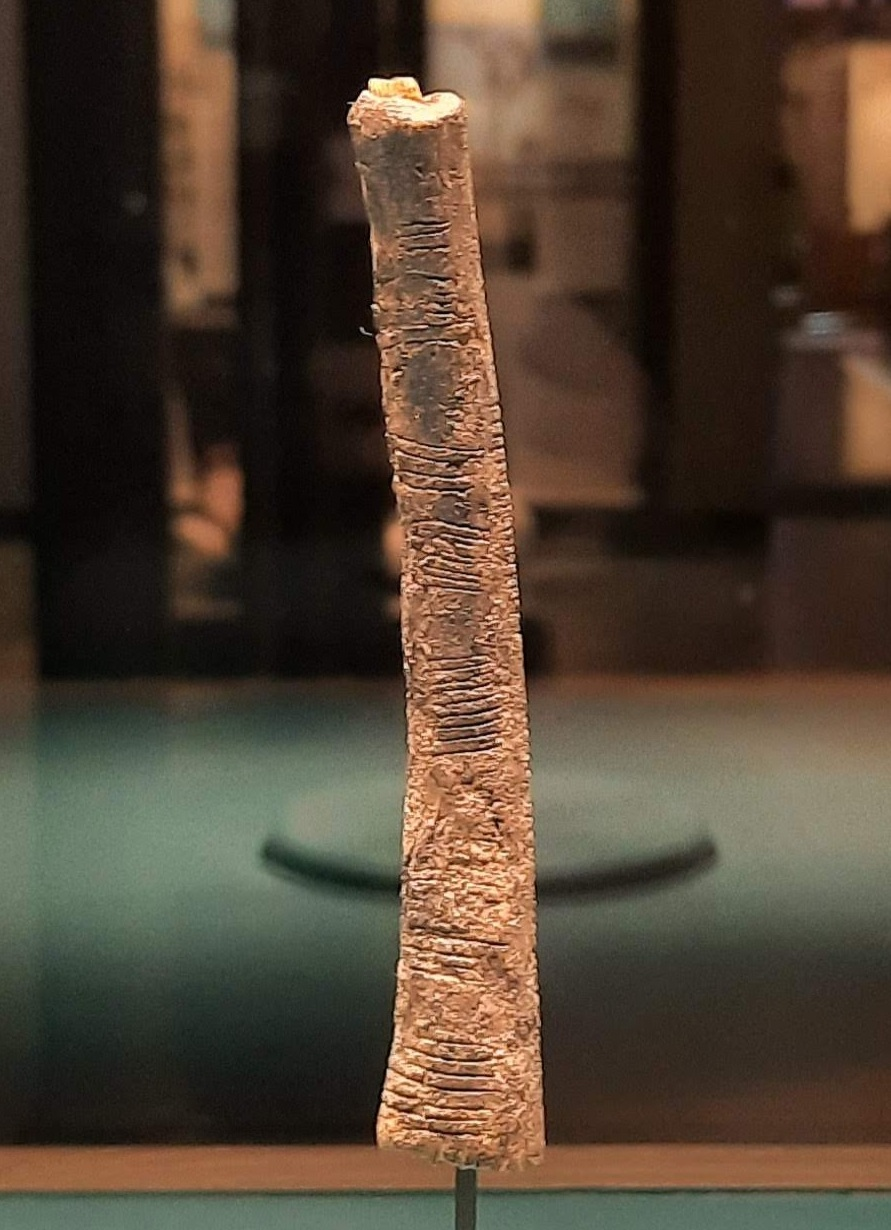
\includegraphics[width=0.45\textwidth]{images/Ishango_bone.jpg}
	\caption{The Ishango bone (photo from Wikimedia).}
	\label{fig:ishango_photo}
\end{figure}

The Ishango bone has three columns of notches arranged in distinct groups. One interpretation suggests these groups represent:
\begin{compactitem}
	\item Column 1: Groups of 3, 6, 4, 8, 10, 5 (demonstrating doubling?)
	\item Column 2: Groups of 11, 13, 17, 19 (prime numbers?)
	\item Column 3: Groups of 11, 21, 19, 9 (numbers around 10 and 20?)
\end{compactitem}

But here's the problem: we don't know what it means.

Was it a tally—a record of objects or events counted over time? Was it a lunar calendar, tracking the phases of the moon? Was it a mathematical exercise demonstrating number relationships? Or was it something we can't even imagine—some cultural practice or record-keeping system lost to history?

The honest answer is: we don't know. And that's important to acknowledge. The archaeological record gives us artifacts, but not intentions. We see the marks; we infer the meaning.

\subsection{The Lebombo Bone: Even Older}

If the Ishango bone is mysterious, the \textbf{Lebombo bone} is even more so. Discovered in 1970 in the Lebombo Mountains of southern Africa, this baboon fibula is broken, but even in its fragmentary state, it bears 29 clearly deliberate notches.

Here's what makes it stunning: it's approximately 43,000 years old.

Think about that timeframe. This bone was marked when Neanderthals still lived in Europe. Modern humans were just beginning to spread across the globe. There was no writing, no cities, no agriculture. But someone—some human being whose name we'll never know—carefully carved 29 notches into a bone and kept it.

Why 29? Some researchers suggest it might track lunar cycles (one lunar month is roughly 29.5 days). Others think it could be a tally of objects, events, or days. Still others caution against over-interpretation: maybe 29 is where the bone broke, and there were originally more notches.

We simply don't know. But here's what we \textit{can} say with confidence:

\begin{keyidea}[What Notched Bones Tell Us]
	Even without knowing their specific purpose, notched bones reveal critical information about early human cognition:
	
	\textbf{1. Intentional marking:} The notches are too regular to be accidental. Someone deliberately created them, one by one, with purpose.
	
	\textbf{2. External memory:} The person didn't rely solely on memory. They offloaded information onto a physical object—a profound cognitive technology.
	
	\textbf{3. Sequential recording:} Notches were added over time, creating a cumulative record. This suggests tracking something that accumulated or recurred.
	
	\textbf{4. Symbolic representation:} Each notch represents something else—an object, event, or unit of time. This is abstract thinking made physical.
\end{keyidea}

\subsection{Why Bones? The Technology of Available Materials}

Modern students sometimes ask: "Why did early humans use bones? Weren't there better materials?"

The answer reveals something important about the relationship between cognition and technology: you work with what you have.

Bones were everywhere in hunting societies—durable animal remains that could be shaped, carved, and carried. They were:
\begin{compactitem}
	\item \textbf{Portable}: Light enough to carry, unlike stone
	\item \textbf{Durable}: Lasted years or decades
	\item \textbf{Workable}: Could be carved with stone tools
	\item \textbf{Available}: Every successful hunt provided them
\end{compactitem}

Other materials might have been used too—wood, bark, leather—but those decay. What survives in the archaeological record isn't necessarily what was most commonly used; it's what's most resistant to time. Bone survives. Wooden tally sticks rot.

This creates a profound problem for archaeology: we're seeing only the tip of the iceberg. For every marked bone preserved over 40,000 years, how many wooden sticks, knotted strings, or sand drawings were used and lost?

The artifacts we have are almost certainly exceptions—the rare survivors of much more widespread practices.

\subsection{The Problem of Interpretation}

Let's be honest about something: interpreting these ancient marks requires immense caution.

Consider the controversy around the Ishango bone. When it was first analyzed, some researchers claimed it demonstrated sophisticated mathematical knowledge—doubling, prime numbers, perhaps even a primitive number base system. Others cautioned that we might be projecting our own mathematical thinking onto random or mundane markings.

Here's the fundamental challenge: \textit{pattern recognition is easy; proving intention is hard}.

Humans are exceptionally good at finding patterns—even in random data. We see faces in clouds, messages in noise, significance in coincidence. So when we look at ancient artifacts, we must ask: are we seeing what was intended, or what we want to see?

The most intellectually honest position acknowledges both possibilities:

\begin{important}[The Archaeological Dilemma]
	\textbf{What we know for certain:}
	\begin{compactitem}
		\item Humans 40,000+ years ago made deliberate, regular marks on durable objects
		\item These marks required effort and intentionality
		\item They were preserved, suggesting value to their makers
		\item Different marks exist in distinct groupings
	\end{compactitem}
	
	\textbf{What we don't know:}
	\begin{compactitem}
		\item The specific purpose of most marked objects
		\item Whether patterns we perceive were intended
		\item What counting systems (if any) were used
		\item How widely such practices spread
	\end{compactitem}
	
	This uncertainty doesn't diminish their importance. It reminds us that the birth of mathematical thinking is shrouded in deep time, accessible only through fragmentary physical traces of vanished minds.
\end{important}

\subsection{The Cognitive Revolution Preserved in Stone}

Despite uncertainties about specific artifacts, the broader picture is clear: between roughly 50,000 and 40,000 years ago, human behavior changed dramatically. Archaeologists call this the \textbf{cognitive revolution} or \textbf{Upper Paleolithic transition}.

Before this period, human tools and artifacts are relatively uniform across vast spans of time. After it, we see explosion of innovation:
\begin{compactitem}
	\item Complex tools with multiple parts
	\item Representational art—cave paintings, carved figurines
	\item Ornamentation and symbolic objects
	\item Evidence of long-distance trade networks
	\item Marked bones and tallying systems
	\item Musical instruments
	\item Elaborate burial practices suggesting abstract thought about death and identity
\end{compactitem}

Something fundamental changed in human cognition. We became fully symbolically fluent—capable of representing abstract concepts, planning across time, and creating external memory systems.

We have focused heavily on the period from roughly 40,000 to 10,000 years ago---the Upper Paleolithic, when notched bones and other artifacts appear in the archaeological record. But we must zoom out and ask a more fundamental question: Why \textit{then}? Anatomically modern humans emerged at least 200,000 years ago. Why did symbolic notation only appear in the last 50,000 years?

\subsection{The Blombos Cave Evidence: Symbolic Thought Before Number}

In 2002, archaeologists working at Blombos Cave in South Africa announced a stunning discovery: a pair of ochre plaques, approximately 75,000 years old, engraved with geometric patterns---cross-hatching, parallel lines, deliberate and repetitive. These are not notches for counting; they are \textit{designs}, patterns created for their own sake. But they demonstrate something critical: the capacity for \textbf{symbolic representation}.

A symbol is an arbitrary mark that stands for something other than itself. The cross-hatched pattern on the Blombos ochre does not resemble anything in nature; it is an abstract design, meaningful only because someone decided it was meaningful. This is the cognitive prerequisite for all notation systems: the ability to create, recognize, and manipulate arbitrary symbols.

Without this capacity, notches are just scratches. With it, notches become \textit{data}. The Blombos evidence suggests that the cognitive hardware for symbolic thought was in place by 75,000 years ago. But it took another 30,000 years for that hardware to be deployed systematically for \textit{quantification}. Why?

\subsection{The Cultural Bottleneck and Population Pressure}

One hypothesis, controversial but compelling, is that symbolic culture---including numerical notation---only becomes \textit{necessary} and \textit{sustainable} when populations are large enough and interconnected enough to support cumulative cultural evolution. In small, isolated bands, innovations are fragile; they can be lost in a single generation if their inventor dies. But in larger, denser populations, innovations spread, persist, and build upon one another.

Around 50,000 years ago, human populations began expanding and intensifying. New technologies appeared: sophisticated stone tools, long-distance trade networks, personal ornaments, cave art. This was the \textbf{Upper Paleolithic Revolution}, and it coincided with the first clear evidence of mathematical notation. Perhaps notches did not appear earlier not because earlier humans were cognitively incapable, but because they lacked the social density and ecological pressure that made notation worth inventing and preserving.

This is speculative, but it aligns with what we know about cultural evolution: complex technologies require not just smart individuals, but smart \textit{societies}.

\begin{connection}[To Modern Computing]
	Every time you write a variable name in code, you're using external memory. The computer doesn't care if you call something \texttt{count} or \texttt{x}—but you do. That symbolic label offloads cognitive burden, letting you think about the concept instead of constantly tracking its specific value.
	
	This is exactly what notched bones did: they offloaded the burden of remembering quantities, freeing up mental resources for other tasks. The principle hasn't changed in 40,000 years—only the technology has improved.
\end{connection}

\section{From Perception to Permanent Record}
\label{sec:perception-to-record}

\begin{sectionintro}
	We've traced the cognitive foundations of number sense and examined the earliest physical evidence of quantitative thinking. Now we must ask: how did humans bridge the gap between perceiving quantity and recording it systematically? This transition—from fleeting mental awareness to permanent external notation—is one of the most consequential developments in human history.
\end{sectionintro}

\subsection{The Problem of Memory}

Try this thought experiment: you're an early human responsible for a small herd of goats—perhaps eight animals. Every morning, you count them as they leave the enclosure to graze. Every evening, you must verify all have returned.

If you have names for numbers (which your language might not), you might think: "Eight this morning, eight tonight—good." But what if you don't have words for eight? Or what if your herd is fifteen goats, and your language only has words for "one," "two," "three," and "many"?

You face a problem: \textbf{working memory is limited}.

Modern cognitive science has shown that human working memory—the mental scratchpad where we hold temporary information—can typically hold about four unrelated items simultaneously. Seven at most, under ideal conditions. Beyond that, without external aids, we start forgetting.

This creates a fundamental bottleneck: if you need to track quantities larger than your working memory capacity, you need external support.

\subsection{External Memory: The First Information Technology}

The solution our ancestors invented was elegant: \textit{if your mind can't hold all the information, store some of it in the world}.

Imagine that goat herder again. Without number words beyond "three," how do you track eight goats? Simple: gather eight pebbles. Each morning, as a goat leaves, move one pebble from your left hand to your right. When all goats are out, all pebbles are transferred. 

In the evening, reverse the process: as each goat returns, move a pebble back. If pebbles remain when the last goat enters, someone is missing. You don't need to count in the modern sense—you've established \textit{one-to-one correspondence} between goats and pebbles.

This is external memory in its simplest form: using physical objects to represent and track information your brain cannot comfortably hold.

The notched bones we discussed earlier are a more sophisticated version of the same idea. Instead of carrying eight separate pebbles (which might be lost), you carry one bone with eight marks. The marks are permanent, cumulative, and portable.

\begin{keyidea}[The Power of External Memory]
	External memory systems transform what humans can accomplish:
	
	\textbf{Extend capacity:} Track quantities far beyond working memory limits
	
	\textbf{Preserve information:} Records persist when memory fails
	
	\textbf{Enable communication:} Physical markers can be shown to others, conveying information without language
	
	\textbf{Support planning:} Marks accumulate over time, enabling long-term tracking
	
	\textbf{Free cognitive resources:} Offloading details to external systems lets you think about higher-level patterns and relationships
\end{keyidea}

\subsection{From Ephemeral to Permanent}

Early external memory systems might have been quite simple and temporary:
\begin{compactitem}
	\item Pebbles arranged in groups
	\item Marks scratched in sand or dirt
	\item Knots tied in grass or vine
	\item Fingers used in specific gestures
\end{compactitem}

These work for immediate, short-term tracking. But they have limitations: pebbles scatter, sand smooths, grass decays, gestures are forgotten.

The move to durable materials—notched bones, marked stones, tied strings that last—represents a crucial transition. Information becomes \textit{persistent}. You can mark a bone today and consult it next week, next month, or next year. You can pass it to someone else, even to future generations.

This persistence changes what's possible. You're no longer limited to information you can personally remember or observations you can personally make. Knowledge begins to accumulate beyond individual lifespans.

\subsection{The Cognitive Cost of Abstraction}

Here's something subtle but important: creating external memory requires abstract thinking.

When you carve a notch to represent a goat, you're doing something conceptually sophisticated. That notch isn't a picture of a goat—it doesn't look like one, doesn't behave like one, doesn't have any goat-like properties. It's purely symbolic. The relationship between mark and meaning exists only in your mind.

This is \textit{representation}—using one thing to stand for another thing based on arbitrary convention. And it's cognitively demanding.

Young children struggle with symbolic representation. A two-year-old doesn't understand that a photo represents a person; they might try to pick up a photographed object. By four or five, children master symbolic thought—understanding that symbols (words, pictures, marks) can represent things that aren't present.

For early humans developing counting systems, every notch required this cognitive leap: this mark represents that thing, even though they share no physical similarity.

\subsection{One-to-One Correspondence: The Foundation of Counting}

Let's return to a concept we mentioned earlier: \textit{one-to-one correspondence}. This is the principle that underlies all counting, all tallying, all systematic quantification.

The idea is simple: two collections are equal if you can pair each item in one collection with exactly one item in the other, with nothing left over.

Example: Do I have the same number of sheep as I have markers?
\begin{compactitem}
	\item Assign one marker to each sheep
	\item If markers remain, I have more markers than sheep
	\item If sheep remain, I have more sheep than markers
	\item If both are exhausted simultaneously, the quantities are equal
\end{compactitem}

Notice something profound: \textit{you never needed to know the actual number}. You didn't need words for "five" or "twelve" or "twenty-seven." You just needed to establish the correspondence.

This is how counting works at its most fundamental level. When you count objects—"one, two, three, four"—you're establishing one-to-one correspondence between number-words and objects. The last number-word you use tells you the total quantity.

But you could do the same thing without number-words, using markers instead. The principle is identical.

\begin{connection}[To Arrays and Indexing]
	One-to-one correspondence is exactly what array indexing does. In an array of size $n$, each index (0 through $n-1$) corresponds to exactly one memory location. No index maps to multiple locations; no location lacks an index.
	
	When you write \texttt{array[5] = value}, you're establishing correspondence: "the element at position 5 gets this value." The index is your marker; the memory location is your object. Different technology, same cognitive principle, 40,000+ years later.
\end{connection}

\subsection{The Social Dimension of Quantification}

We've focused on cognitive and technological aspects, but there's another crucial dimension: \textit{social pressure}.

As human groups grew larger and more complex, the need for systematic quantification intensified:

\textbf{Resource distribution:} Fair division requires measuring and comparing. Who gets what portion? How do we split resources equitably?

\textbf{Trade and exchange:} Trading across groups requires agreed-upon values. Three of my baskets for five of your tools—but only if we can count reliably.

\textbf{Social obligations:} Who owes whom? Keeping track of debts, favors, and obligations requires memory—often external memory.

\textbf{Collective planning:} When should we move camp? How many days until the rains come? How many people can we feed through winter?

\textbf{Status and hierarchy:} Prestige might come from possessing more—more livestock, more tools, more stored food. But "more" must be quantifiable and comparable.

These social pressures created evolutionary advantage for groups with better quantification systems. Groups that could track, plan, trade, and coordinate effectively outcompeted those that couldn't.

Mathematics, in this view, is a social technology as much as a cognitive one. It emerges from our need to cooperate, communicate, and organize collectively.

\subsection{The Path Forward}

We've now established the foundations:
\begin{compactitem}
	\item Humans possess innate number sense—the ability to perceive and compare quantities
	\item We made a cognitive leap to \textit{representation}—thinking abstractly about quantity
	\item We developed external memory systems—marks, tokens, physical representations
	\item We established one-to-one correspondence—the logical foundation of all counting
	\item Social complexity created pressure for better quantification systems
\end{compactitem}

These aren't just historical curiosities. They're the cognitive and cultural foundations on which all subsequent mathematics built. When Mesopotamians developed place-value notation, when Greeks proved geometric theorems, when medieval algebraists solved equations, when modern computer scientists design algorithms—all of it rests on these ancient cognitive achievements.

In the next chapter, we'll see how these primitive beginnings evolved into more sophisticated systems: body counting, finger mathematics, and the extraordinary diversity of ways human cultures have represented quantity. But the foundation remains the same: the drive to understand, represent, and manipulate quantity—a drive that transformed our species and ultimately gave us mathematics itself.
\newpage
\begin{motivation}[Why This Matters for Computer Science]
	You might wonder: why does a computer science student need to know about 40,000-year-old bones and prehistoric cognition?
	
	Because \textit{the principles haven't changed}.
	
	When you design a data structure, you're solving the same problem ancient humans solved: how to represent information efficiently so it can be stored, retrieved, and manipulated. When you choose between arrays, linked lists, or hash tables, you're making decisions about external memory—just like choosing between notched bones, piled pebbles, or knotted strings.
	
	The technology differs. The mathematics grew more sophisticated. But the fundamental challenge remains: taking something abstract (quantity, relationship, information) and representing it concretely so both humans and machines can work with it.
	
	Understanding these origins isn't just historical appreciation—it's conceptual foundation. When you grasp why external memory matters, why one-to-one correspondence is fundamental, why symbolic representation requires cognitive effort, you understand data structures at a deeper level.
	
	Every array you create is a descendant of those first notched bones. Every algorithm you write relies on principles discovered by people who never heard the word "algorithm." The past illuminates the present—and prepares you for the future.
\end{motivation}

\begin{center}
	\decorativeseparator
\end{center}

\textit{In the next chapter, we explore how humans moved beyond simple tallying to develop richer notation systems using the most readily available tool: the human body itself. We'll trace the development of finger counting and body-part enumeration systems that persist in some cultures to this day, and examine why our hands have shaped mathematics in ways that echo through modern number systems.}